\chapter{Proposed Method}
\label{ch:proposal}

In this thesis, we present a new algorithm for colour correction. We take the polynomial regression model further by utilising piecewise polynomials, specifically splines. The piecewise property enables polynomials of varying smoothness to be fitted across the function domain. Although different types of splines exist, basis splines (B-splines) are often used due to their minimal support, which means they can be fitted locally. This allows us to restrict sharp changes in the function shape to a restricted domain, unlike with polynomials \cite[140]{HastieTrevor2009EoSL}.

The idea of using splines for colour correction came upon reading \cite{finlayson2015color}. An observation of the smoothness of the fit was particularly emphasised, which is why they initially proposed the root polynomial model. The idea was based on the fact that reflectance spectra are usually relatively smooth, and linear models already perform exceptionally well. Furthermore, the spectral sensitivities of an image sensor and cones are relatively close, so a good fit is achievable with little non-linearities. Similar observations, albeit for scanners, were also discussed in \cite{wandell1993water}.

\section{Splines}

Splines belong to the family of piecewise polynomials but have constraints that make them convenient for fitting smooth functions. The boundary of each interval is known as a \textbf{knot}. For regular piecewise polynomials, the function values at knots are not constrained, and thus we may run into discontinuities \cite[141-144]{HastieTrevor2009EoSL}. This effect is shown in the top left plot in Figure \ref{fig:discontinuity}, where age is plotted against wage. At $Age=50$, there is an apparent discontinuity in the fitted function, although it still captures the shape of the data well.

In the top right plot in Figure \ref{fig:discontinuity}, we see another attempt to fit a polynomial to the data, but this time with a constraint that the two functions must be joined at the knot, making it continuous. This, however, creates a corner at $Age=50$, and the analytical derivative is not defined at that point. Consequently, the function is not very smooth at this point.

\begin{figure}
    \centering
    \pdftooltip{\includegraphics[width=\textwidth]{figures/7_3.pdf}}{piecewise polynomial}
    \caption{Piecewise polynomial fit with discontinuity \cite[295]{JamesGareth2023AItS}.}
    \label{fig:discontinuity}
\end{figure}

Finally, two spline model fits are shown at the bottom of Figure \ref{fig:discontinuity}. For a degree $d$ spline ($d=33$ for cubic, $d=1$ for linear), there is a constraint that the derivatives are continuous up to degree $d-1$ \cite[296]{JamesGareth2023AItS}, \cite[187]{HastieTrevor2009EoSL}. For the left plot, we thus have a guarantee that all derivatives up to degree 2 are continuous. In contrast, for the linear spline in the right figure, we only have a requirement that the function's first derivative is continuous, which is accurate as it is just a constant.

The order and the knots thus parametrise splines. For the former, there are two parameters we can tune: the position and number of the knots. The choice of location of the knots usually depends on whether we have some domain knowledge about the problem, e.g., knowing the locations of abrupt changes in the function. Otherwise, the knots can be placed at uniform distances or based on the data distribution (quantiles). The number of knots can be chosen similarly from the assumptions of the function shape  \cite[186-189]{HastieTrevor2009EoSL}.

\subsection{B-splines}

Perhaps the most important family of spline functions is formed by \textbf{basis splines}, commonly known as B-splines. The name comes from the fact that all other types of splines can be approximated by linear combinations of B-splines, acting as a basis for the family of splines.\cite[87-93]{practicalguidetosplines} An example of a different order B-splines was seen in the bottom row of \ref{fig:discontinuity}, where 3rd and 1st order functions were used respectively.

As stated before, all B-spline functions are defined as a linear combination of lower-order splines. Unlike polynomials, a spline of order $M$ consists of polynomials of degrees $M-1$ due to the continuity condition at the knots. Increasing order of B-splines can then be computed recursively given the first-order spline formula:

\begin{equation}
B_{i,1}(x) = 
\begin{cases} 
1 & \text{if } \tau_i \leq x < \tau_{i+1} \\
0 & \text{otherwise}
\end{cases}
\end{equation}

\text{for } i = 1, \ldots, K + 2M - 1, where $K$ is the number of knots and $\tau_i$ and $\tau_{i+1}$ denote the \textbf{support} of the function. Generally, a spline of order $M$ also spans $M$ knots, and thus, for a 1st order spline, we have that the constant function spans a single knot \cite[186-189]{HastieTrevor2009EoSL}.

A B-spline of order $M$ is the sum of two shifted order $M-1$ B-splines at the current knot position $i$ and the next knot position $i+1$. The formula is then given by: 
\begin{equation}
\label{formula:splines}
B_{i,m}(x) = \frac{x - \tau_i}{\tau_{i+m-1} - \tau_i} B_{i,m-1}(x) + \frac{\tau_{i+m} - x}{\tau_{i+m} - \tau_{i+1}} B_{i+1,m-1}(x)
\end{equation}
\text{for } i = 1, \ldots, K + 2M - m. \cite[186-189]{HastieTrevor2009EoSL}, \cite[90]{practicalguidetosplines}.

Figure \ref{fig:spline} displays the first three B-spline functions of non-zero order. As in equation \ref{formula:splines}, the splines recursively utilise adjacent lower-order splines in the formation, it can be observed that the higher-degree splines are also non-zero for a wider area. This is also apparent from the property that a nth order spline spans $M+1$ knots and is also evident from formula \ref{formula:splines}, where the subsequent interval is also always considered.

\begin{figure}
    \centering
    \pdftooltip{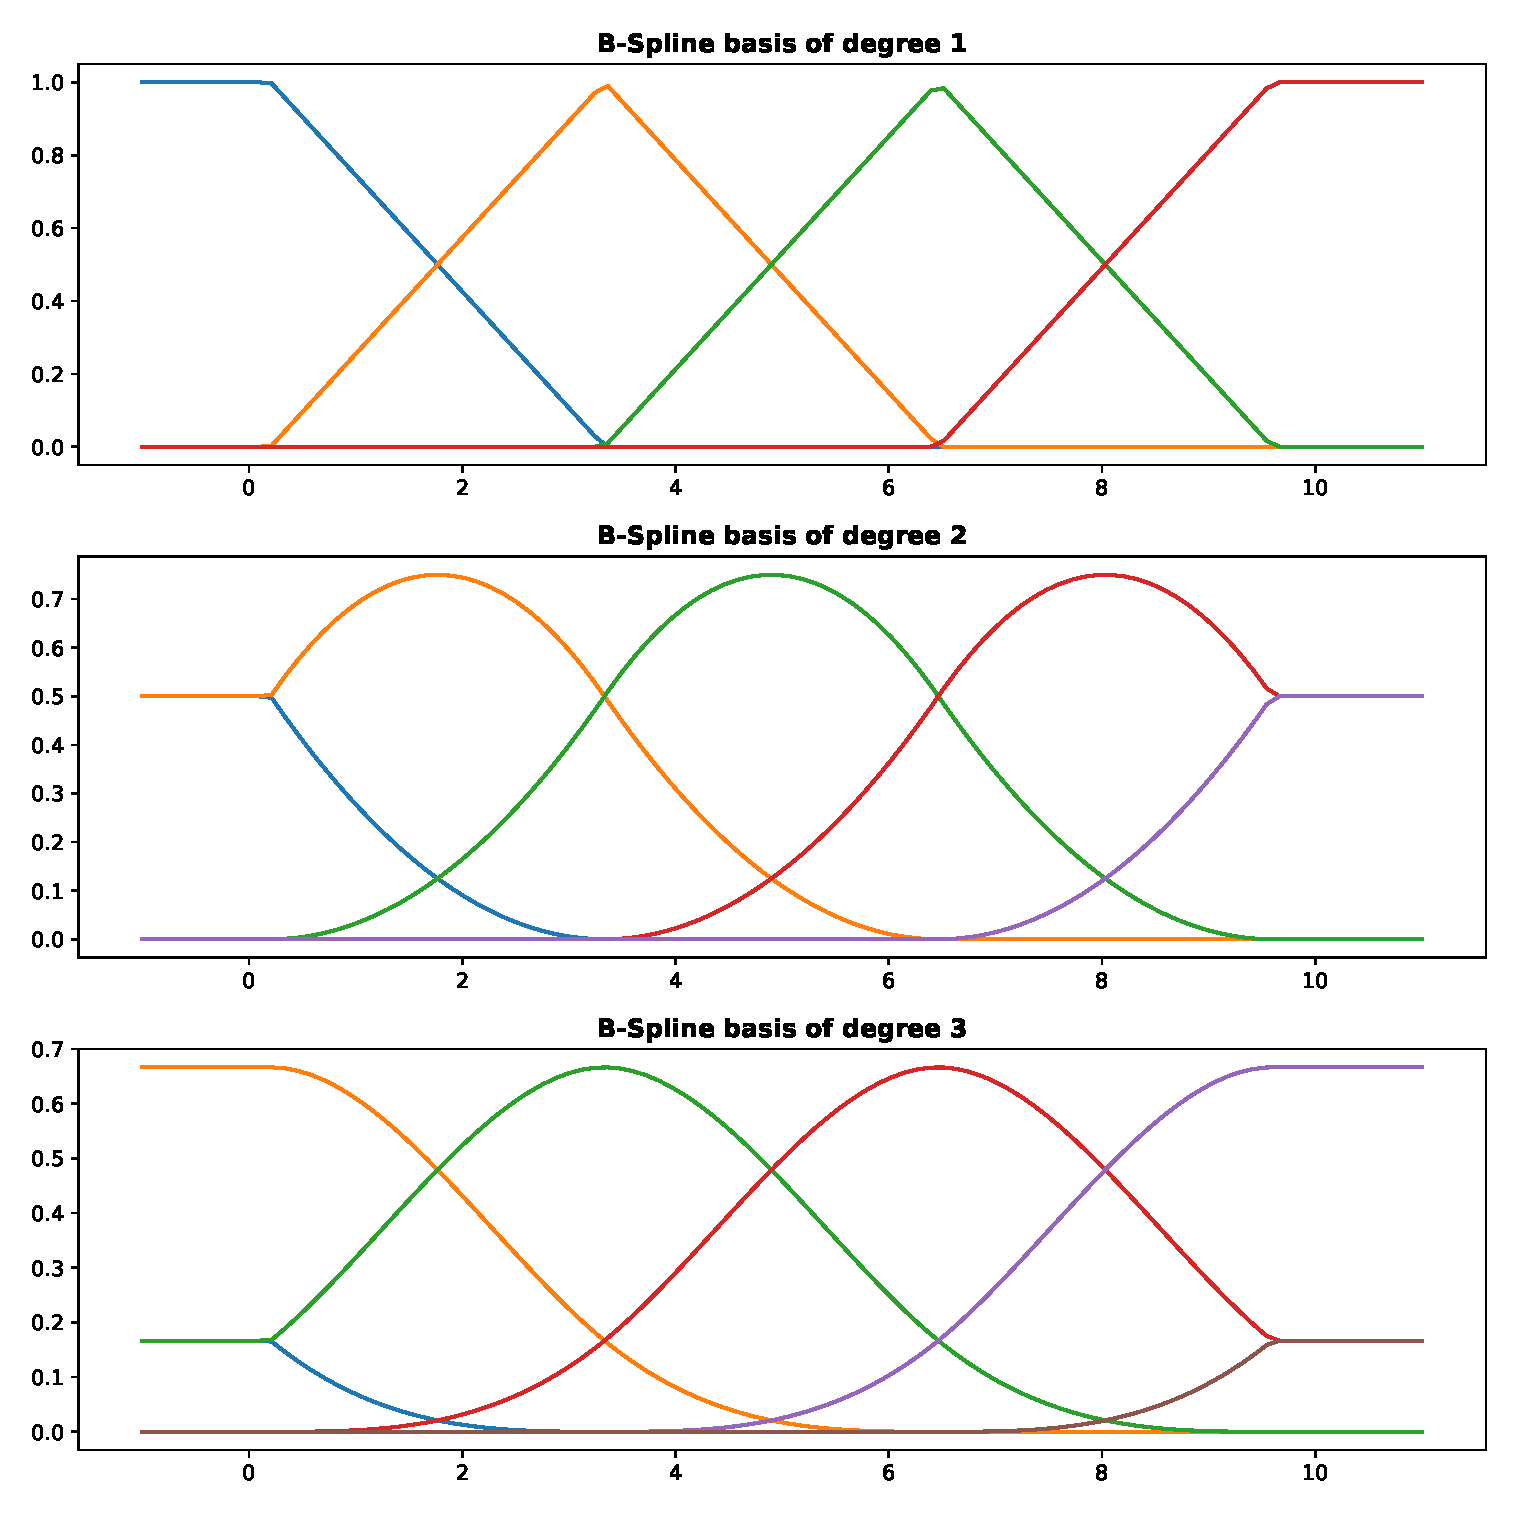
\includegraphics[width=\textwidth]{figures/splines.eps}}{B-Spline basis functions}
    \caption{Spline basis functions visualised}
    \label{fig:spline}
\end{figure}

Theoretically, this should allow us to approximate a large family of functions with linear combinations of B-splines. For example, in regression problems, we can utilise basis transformations of the original variables as new features. The output is then a linear combination of the B-spline features and may well approximate another spline function without us explicitly finding the correct basis.

\subsection{Tensor Product Splines}

As was seen in \ref{ss:polynomials}, polynomial models often utilise interactions between the original features as new features. This is carried out by a simple multiplication of the features. Up to two variables, these can be visualised as surface approximating the target output, which offers intuition on the nature of the fit.

Utilising interactions between variables, as was done with polynomial models, is also straightforward with splines via tensor products. Assuming we have transformed our red and green channel features using $n$ splines per feature, the interactions would be captured as follows:

\begin{equation}
\label{tensorspline}
\mathbf{r} \otimes \mathbf{g} = \mathbf{r} \mathbf{g}^T =
\begin{pmatrix}
r_1 g_1 & r_1 g_2 & r_1 g_3 \\
r_2 g_1 & r_2 g_2 & r_2 g_3 \\
r_3 g_1 & r_3 g_2 & r_3 g_3 \\
\end{pmatrix},
\end{equation}
where $\mathbf{r}$ and $\mathbf{g}$ are $n \times 1$ vectors containing the values of the $n$ B-spline basis evaluated at the position of the input pixel's intensity level for the red and green channels. All two-way interactions can then be considered using three tensor-product matrices: $\mathbf{r} \otimes \mathbf{g}$, $\mathbf{r} \otimes \mathbf{b}$ and $\mathbf{g} \otimes \mathbf{b}$. Combining these into one matrix forms our design (or basis) matrix for regression.

The beauty of this is that we can now assign each tensor product term its term and control the shape of the regression surface more effectively. An example of a surface generated by a tensor product spline of two variables can be seen in Figure \ref{fig:tensorspline}.

A downside to tensor product splines is the curse of dimensionality \cite[163]{HastieTrevor2009EoSL}. As we increase the number of features or splines per feature, the dimension of our feature matrix increases quadratically. In practical implementations, especially when running on low-power embedded devices, there is thus a trade-off between possible performance gains and computing resources. 

\begin{figure}
    \centering
    \pdftooltip{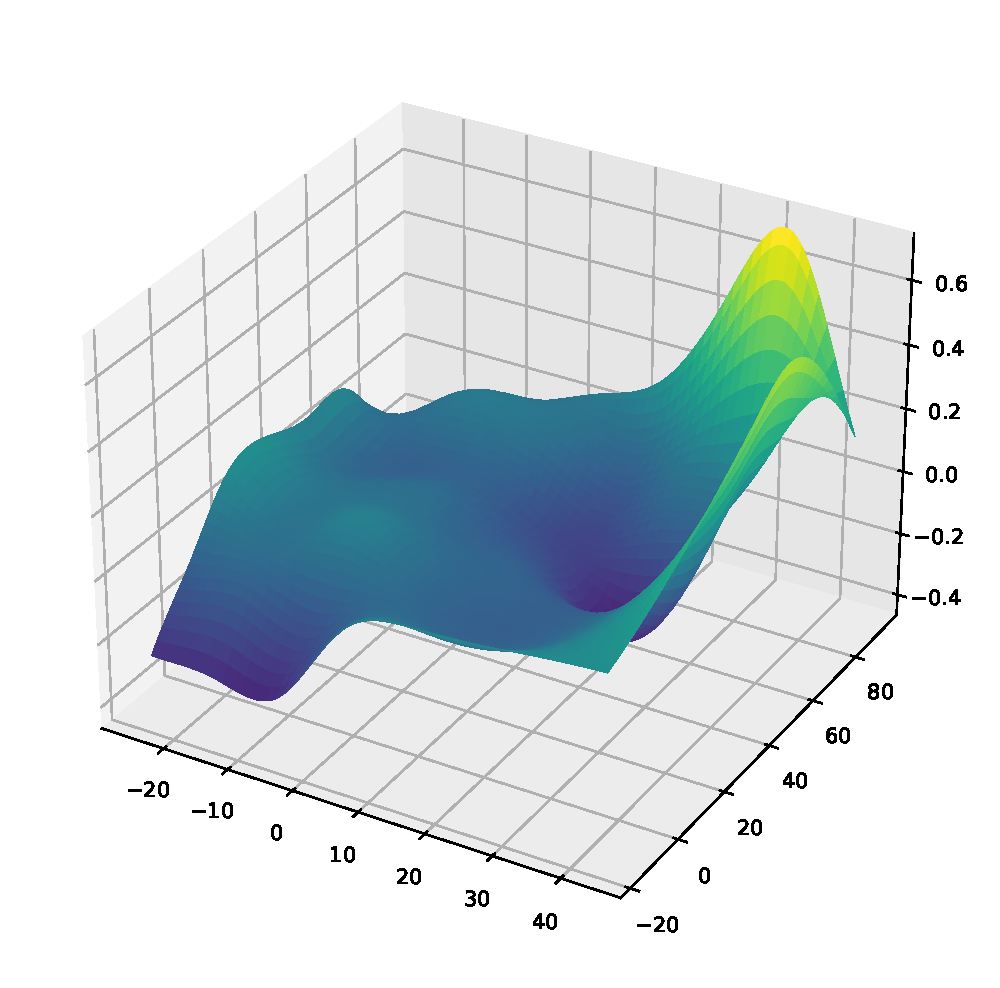
\includegraphics[scale=0.7]{figures/tensorspline.eps}}{Tensor Product Splines}
    \caption{Partial dependence visualisation of a tensor product spline term.}
    \label{fig:tensorspline}
\end{figure}

\section{Penalised B-splines for Colour Correction}

The primary research output of this thesis is the use of an extension of B-splines, known as Penalised B-splines. In the previous section, we saw how splines allow us to extend our basis into a new one with fine-grained control through piecewise polynomials. We also discussed how the dimension of the basis grows exponentially when we introduce interactions between splines. Here, we introduce the origins and theory behind our model.

\subsection{Model Regularization}

An issue commonly discussed in the Machine Learning (ML) communities is overfitting. This happens when the model is too complex and begins to fit precisely to the data points in our training set. Often, this is not desired, as the training data is just a subset of the samples we see in the real world, and the surface might fit poorly to unseen data. Often, the way to combat this is to increase data by collecting more real-world samples or augmenting the data, for example, by adding noise to the existing samples. This effect is visible in Figure \ref{fig:overfit}, where an overly complex polynomial model is fit to noisy sinusoidal data.

Another way to prevent overfitting is by introducing a penalty term to the least-squares problem. 
This is called regularisation, and often methods are used, such as Ridge \cite{hoerl2000ridge} and Lasso \cite{tibshirani1996regression} regression. They minimise the coefficients' L2 and L1 norms, resulting in a more numerically stable range of values for coefficients, especially for models where the features are correlated.\cite[61-69]{HastieTrevor2009EoSL} In these cases, we often observe large coefficients when using regular least-squares techniques.

\begin{figure}
    \centering
    \pdftooltip{\includegraphics[scale=0.8]{figures/overfit.eps}}{Example of overfitting}
    \caption{Example of a high-degree polynomial model overfitting a noisy sinusoidal data}
    \label{fig:overfit}
\end{figure}

Another way to regularise a regression model with many predictors is to penalise the second derivative of our predictors. Second derivatives correspond to the curvature of our function, and as such, the penalisation term attempts to fit a line or a hyperplane to the data. Often these are paired with least-squares objective, which attemps to interpolate the training data. The balance between these two is determined by the smoothing parameter $\lambda$ in the following way:

\begin{equation}
\text{RSS}(f, \lambda) = \sum_{i=1}^{N} \left\{ y_i - f(x_i) \right\}^2 + \lambda \int \left\{ f''(t) \right\}^2 dt,
\label{formula:smoothingsplines}
\end{equation}

where $y_i$ are the target samples, $f(x_i)$ are the interpolating functions, and $\lambda$ controls the effect of the penalty term on the loss. These are often called Smoothing Splines, although $f(x_i)$ can also be any other function and is picked based on which minimises the loss. \cite[151]{HastieTrevor2009EoSL}

\subsection{Penalized B-Splines}

Penalised B-splines (P-Splines) were first proposed by \citeauthor{eilers1996flexible} in 1996 \cite{eilers1996flexible}. Their formulation is similar to that of smoothing splines in \ref{formula:smoothingsplines}, but they instead penalise the difference of coefficients in adjacent splines. They are then defined as follows:

\begin{equation}
\|\mathbf{y} - \mathbf{B}\boldsymbol{\alpha}\|^2 + \lambda \|\mathbf{D}\boldsymbol{\alpha}\|^2,
\label{formula:psplines}
\end{equation}

where $\lambda$ again controls the penalty term, $\mathbf{B}$ and ${\alpha}$ are the design matrix of basis functions and coefficients. $\mathbf{D}$ is known as the difference matrix, and multiplying $\alpha$ with it computes the nth order differences of $\alpha$. For example, the first-order difference between adjacent coefficients would be $(\alpha_j - \alpha_{j-1})^2$. \cite{eilers2021psplines}

With P-splines, it does not harm to have a too large basis if computational complexity is not a concern. Selecting the smoothing parameter appropriately is quickly done by a simple grid search. In Figure \ref{fig:largebasis} we see this property of P-splines in action, with the basis functions scaled by their coefficients in different colors. Despite the number of basis functions being much larger than the number of training samples, the produced curve is smooth and does not overfit the data. It is thus safe to pick excessively too many basis functions initially, visualise the produced surface and restrict their number if the computation becomes a bottleneck. \cite{eilers2021psplines} An initial model might act as a starting point for analysing the nature of the transformation at hand before any optimisations.


\begin{figure}
    \centering
    \pdftooltip{\includegraphics[scale=0.5]{figures/pspline_smoothing.png}}{Example of using a large basis with P-splines}
    \caption{Example of using a large basis with P-splines. Visualized using P-spline Playgrounds\cite{psplinesJoysPsplines}.}
    \label{fig:largebasis}
\end{figure}

\subsection{Proposed solution}

Based on the presented theory, a proposed model uses tensor product splines combined with the P-spline penalty. We can model more complex surfaces that relate the RGB values to the target XYZ values by considering the interactions between variables at different intervals. However, unlike in interpolation, we do not limit ourselves to passing through the points in the training data, which gives us flexibility in the training process.

Figure \ref{fig:partialdep} shows the tensor product partial dependences on $Y$ for all red, green and blue combinations on a model trained using Nikon D5100 spectral sensitivities. The knots formed by the tensor product can be seen as red dots in the figure. Although we have a function with many basis functions and thus control points, the function still produces a smooth surface as an output, thanks to the penalty term. Note that here, we intentionally fit too many splines to demonstrate the fact that overfitting is not a problem with appropriately chosen $\lambda$, as is suggested by the inventors of the P-spline model \cite{eilers2021psplines}. Since the solution utilises a large basis, it also simplifies the problem of choosing knot positions. Instead, we can place them uniformly, and the least-squares fit will automatically give less weight to the basis functions, which would not contribute either way.

\begin{figure}
    \centering
    \pdftooltip{\includegraphics[width=\textwidth]{figures/partial.png}}{P-Spline predictors}
    \caption{Partial dependences on $Y$ with $\lambda = 0.1$ and 10 basis functions for Nikon D5100.}
    \label{fig:partialdep}
\end{figure}

Thus, our proposed model utilises distinct two-way interactions between the red, green, and blue channels transformed by third-order spline functions. The complexity of our model directly scales with the number of spline basis functions per feature:  for each of the three output channels, three tensor product features are used, resulting in total $3\times 3 \times n^2=9n^2$ terms. Models with 5, 10 and 20 have dimensionality of 225, 900 and 3600, respectively.

The model is simple to build, and many programming languages already offer the required building blocks, such as B-spline basis functions, and support matrix operations, such as tensor (Kroenecker) products and matrix multiplications. For example, one can use pyGAM \cite{serven2018pygam} in Python, mgcv \cite{wood2001mgcv}, or JOPSplus \cite{psplinesJoysPsplines} in R, or the Curve Fitting Toolbox \cite{MatlabCurveFitting2024} in MATLAB. The design matrix of basis functions is also efficient to compute via cardinal b-splines.